% !TEX root = ../../../main.tex

\toggletrue{image}
\toggletrue{imagehover}
\chapterimage{Types}
\chapterimagetitle{\uppercase{Types}}
\chapterimageurl{https://xkcd.com/1537/}
\chapterimagehover{colors.rgb("blue") yields "\#0000FF". colors.rgb("yellowish blue") yields NaN. colors.sort() yields "rainbow"}

\chapter{Typen}
\label{chapter-typen}

Wir schauen uns noch einmal die Berechnungen (Flächeninhalt und Umfang) am Quadrat an. Bei diesem Programm soll nun der Benutzer die Seitenlänge über eine Benutzereingabe angeben können. Das Programm aus \autoref{lst-calc-input-quad-wrong} versucht, dies zu realisieren.

\begin{lstlisting}[language=python, caption={\graybgtexttt{quadrat\_berechnungen\_input.py}}, label=lst-calc-input-quad-wrong]
a = input("Bitte eine Seitenlänge eingeben: ")
umfang = 4 * a
print(<@\color{textcolor}f@>"Umfang: <@\color{keywordcolor}\{\color{black}umfang\color{keywordcolor}\}@>")
flaeche = a ** 2
print(<@\color{textcolor}f@>"Umfang: <@\color{keywordcolor}\{\color{black}flaeche\color{keywordcolor}\}@>")
\end{lstlisting}

Wenn wir das Programm ausführen, dann erhalten wir in der Konsole eine Fehlermeldung, wie in \autoref{lst-calc-input-quad-wrong-output} zu sehen. Das Programm wird noch teilweise ausgeführt, bevor es mit einer Fehlermeldung abstürzt. Die Fehlermeldung gibt uns einen Hinweis darauf, wo und warum das Programm abgestürzt ist.

\begin{lstlisting}[language=output, label={lst-calc-input-quad-wrong-output}, caption={Konsolenausgabe des fehlerhaften Programms.}]
Bitte eine Seitenlänge eingeben: 50
Umfang: 50505050
Traceback (most recent call last):
  File ".../quadrat_berechnungen_input.py", line 4, ...
    flaeche = a ** 2
TypeError: unsupported operand type(s) for ** or pow(): 
  'str' and 'int'

Process finished with exit code 1
\end{lstlisting}

Obwohl wir in der Konsole eine Zahl eingegeben haben, wird das Programm nicht korrekt ausgeführt. Warum? In diesem Kapitel klären wir diese Frage. Dazu müssen wir verstehen, wie Zahlenwerte und Textwerte in Python unterschieden werden. Die Lernziele lauten:

\newcommand{\typenLernziele}{
\begin{todolist}
\item Sie verwenden die passende eingebaute Funktion, um in Python aus einem Textwert einen Zahlenwert zu konstruieren.
\item Sie erklären, was ein Typ ist.
\item Sie bestimmen für einen Wert den dazugehörigen Typ.
\end{todolist}
}

\lernziel{\autoref{chapter-typen}, \nameref{chapter-typen}}{\protect\typenLernziele}

\typenLernziele

\section{Zahlenwerte versus Textwerte}

Im Programm aus \autoref{lst-calc-input-quad-wrong} werden zwei Berechnungen durchgeführt. Die erste Berechnung wird nicht korrekt durchgeführt und die zweite Berechnung bringt das Programm zum Absturz.

\begin{itemize}
\item Das Programm gibt für den Umfang das Ergebnis \lstinline{50505050} aus anstatt \lstinline{200}. Es wird also keine gewöhnliche Multiplikation durchgeführt.
\item Das Programm gibt mit einer Fehlermeldung aus, dass die Potenz nicht berechnet werden kann (Zeile \num{4}).
\end{itemize}

\subsection{Wo liegt der Fehler?}

Es ist ein \textbf{Programmierfehler}. Obwohl wir eine Zahl für die Benutzereingabe eingetippt haben, erkennt Python dies \textbf{nicht} als \textbf{Zahlenwert}, sondern als \textbf{Textwert}! Deshalb ist die erste Berechnung \say{komisch} und die zweite Berechnung nicht möglich. Python \say{versucht}, mit einem Textwert zu rechnen. Warum erkennt Python die Eingabe nicht als Zahl?

\begin{important}
Der \lstinline{input}-Funktionsaufruf liefert die Benutzereingabe über die Konsole. Python betrachtet die Benutzereingabe \textbf{immer} als Text. Selbst dann, wenn wir eine Zahl eingeben, wird dies von Python als Text behandelt.
\end{important}

Python sieht in unserer Eingabe aus \autoref{lst-calc-input-quad-wrong-output} somit nicht die Zahl \lstinline{50}, sondern einen Text mit den Zeichen \texttt{5} und \texttt{0}. Wir müssen Python also dazu bringen, dass wir aus einem Text eine Zahl konstruieren können.

\subsection{Wie beheben wir den Fehler?}

Glücklicherweise ist dies ein Standardproblem und Python besitzt mit \lstinline{int} bereits eine passende Funktion. Mit dieser Funktion können wir aus einem Text eine \textbf{ganze Zahl} konstruieren. \autoref{lst-int-example-1} zeigt ein Beispiel und \autoref{lst-int-example-1-output-1} eine passende Konsolenausgabe.

\begin{lstlisting}[language=python, caption={In Zeile \num{2} wird eine ganze Zahl konstruiert (\graybgtexttt{quadratzahl\_input.py}).}, label={lst-int-example-1}]
eingabe = input("Eine ganze Zahl bitte: ")
zahl = int(eingabe)
quadratzahl = zahl ** 2
print(<@\color{textcolor}f@>"Die Quadratzahl von <@\color{keywordcolor}\{\color{black}zahl\color{keywordcolor}\}@> ist <@\color{keywordcolor}\{\color{black}quadratzahl\color{keywordcolor}\}@>.")
\end{lstlisting}

\begin{lstlisting}[language=output, caption={Beispielausführung für das Programm aus \autoref{lst-int-example-1} mit gültiger Eingabe.}, label={lst-int-example-1-output-1}]
Eine ganze Zahl bitte: 42
Die Quadratzahl von 42 ist 1764.
\end{lstlisting}

\section{Die \lstinline{int}-Funktion}

Diese eingebaute Funktion \textbf{versucht} aus einem Text eine ganze Zahl zu konstruieren. Beim Funktionsaufruf muss das Argument also ein Text sein, der eine Zahl darstellt.

$$
\begin{array}[t]{ccc} 
\underbrace{\textrm{\texttt{zahl}}}_{\textrm{Variable speichert eine ganze Zahl}} & \textrm{\texttt{=}} & \underbrace{\texttt{int(}\underbrace{\textrm{\texttt{eingabe}}}_{\textrm{Variable speichert einen Text}}\texttt{)}}_{\textrm{Erzeugt aus dem Inhalt der Variablen eine ganze Zahl}}
\end{array}
$$

Wir verwenden mit Absicht das Wort \say{versuchen}, da beim Funktionsaufruf auch ein Text benutzt werden kann, welcher nicht eine Zahl darstellt. Falls die Konstruktion einer Zahl nicht möglich ist, dann wird ein Fehler erzeugt und das Programm stürzt ab (siehe \autoref{lst-int-example-1-output-2}).

\begin{lstlisting}[language=output, caption={Beispielausführung für das Programm aus \autoref{lst-int-example-1} mit falscher Eingabe.}, label={lst-int-example-1-output-2}]
Eine ganze Zahl bitte: Apfel
Traceback (most recent call last):
  File ".../quadratzahl_input.py", line 2, in <module>
    zahl = int(eingabe)
ValueError: invalid literal for int() with base 10: 'Apfel'
\end{lstlisting}

\vspace{-0.5cm}

\subsection{Wie kann man die \lstinline{int}-Funktion aufrufen?}

Die eingebaute \lstinline{int}-Funktion kann sehr vielseitig eingesetzt werden. Standardmässig erwartet der Funktionsaufruf \textbf{ein} Argument. Das Argument ist ein Textwert, welcher eine \textbf{ganze Zahl} im \textbf{Dezimalsystem} darstellt. 

\begin{example}
Beispiele für \textbf{gültige} Funktionsaufrufe:
\begin{itemize}
\item \lstinline{lieblingszahl = int("42")}: wandelt das Literal \lstinline{"42"} in die ganze Zahl \lstinline{42} um.
\item \lstinline{ganze_zahl = int(3.14)}: wandelt die Fliesskommazahl \lstinline{3.14} in die ganze Zahl \lstinline{3} um.
\item \lstinline{anzahl_tage = int(input("Countdown in Tagen: "))}: kombiniert die Benutzereingabe mit dem \lstinline{int}-Funktionsaufruf.
\end{itemize}
\end{example}

\vspace{-1cm}

\section{Aufgaben}

In den folgenden Aufgaben setzen Sie sich mit der \lstinline{int}- und \lstinline{float}-Funktion auseinander.

\subsection{Aufgabe 1}

Korrigieren Sie das Programm aus dem Eingangsbeispiel (Berechnung des Umfangs und der Fläche). Sie können die passende Code-Zeile direkt in \autoref{lst-int-float-aufgabe-1} einfügen.

\begin{lstlisting}[language=python, caption={\graybgtexttt{quadrat\_berechnungen\_input.py}}, label=lst-int-float-aufgabe-1]
eingabe = input("Bitte eine Seitenlänge eingeben: ")
# TODO: Wert in der Variablen eingabe in eine ganze Zahl
# umwandeln und in der Variablen a speichern.

umfang = 4 * a
print(<@\color{textcolor}f@>"Umfang: <@\color{keywordcolor}\{\color{black}umfang\color{keywordcolor}\}@>")
flaeche = a ** 2
print(<@\color{textcolor}f@>"Umfang: <@\color{keywordcolor}\{\color{black}flaeche\color{keywordcolor}\}@>")
\end{lstlisting}

\subsection{Aufgabe 2}

Notieren Sie ein Programm, welches mit der Turtle ein Quadrat zeichnet. Der Benutzer soll die Seitenlänge des Quadrats über eine Benutzereingabe selbst bestimmen können.

\fillwithgrid{\stretch{1}}

\newpage

\subsection{Aufgabe 3}

Notieren Sie ein Programm, welches von drei Schulnoten das arithmetische Mittel (\say{Durchschnitt}) berechnet und in der Konsole ausgibt. Man soll auch Noten mit einem \say{Komma} eingeben können. Dazu muss man in \textbf{Python den Punkt} und die eingebaute Funktion \lstinline{float} statt \lstinline{int} verwenden. Die Ausgabe in der Konsole sollte dann wie folgt lauten:

\begin{lstlisting}[language=output]
Note 1: 5.5
Note 2: 3.25
Note 3: 6
Ihr Notenschnitt ist 4.916666666666667.
\end{lstlisting}

Die Noten sind nur ein Beispiel. Das Programm muss für drei beliebige Noten funktionieren.

\fillwithgrid{2.5in}

\subsection{Aufgabe 4}

Notieren Sie ein Programm, welches ein \say{gekipptes Quadrat} gemäss \autoref{figure-aufgabe-gekipptes-quadrat} zeichnet. Der Benutzer soll folgende drei Eigenschaften über die Benutzereingabe wählen können:

\begin{itemize}
\item Neigung des Quadrats: Winkel $\alpha$ des Quadrats in Grad (\say{Kommazahl} soll möglich sein).
\item Seitenlänge des Quadrats (nur eine ganze Zahl soll möglich sein)
\item Farbe der Linien
\end{itemize}

\begin{figure}[htb]
\centering
\begin{minipage}{0.65\textwidth}
\centering
\fillwithgrid{2.5in}
\end{minipage}
\hfill
\begin{minipage}{0.3\textwidth}
\centering
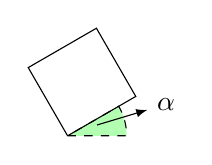
\begin{tikzpicture}
	\draw[fill=green!30, thin, dashed] (0,0) -- ++(0:0.75cm) arc (0:30:.75cm) -- (0,0);	
	\draw (0,0) -- ++(30:1cm) --++(120:1cm)--++(210:1cm) --++(300:1cm);
	\node (A) at (0.25,0.1) {};
	\node (B) at (1.25, 0.4) {$\alpha$};
	\draw[-latex] (A) -- (B);
\end{tikzpicture}
\caption{Gekipptes Quadrat.}
\label{figure-aufgabe-gekipptes-quadrat}
\end{minipage}
\end{figure}

\section{Typisierung}

Während der Ausführung eines Python-Programms muss entschieden werden, ob eine Operation (z.B. Addition) durchgeführt werden kann oder nicht. Dazu ordnet Python jedem Wert (eng. value) eine \say{Kategorie} zu. In Python nennt sich dieser Vorgang \textbf{Typisierung} und der Fachbegriff für die \say{Kategorien} nennt sich \textbf{Typen}.

\begin{definition}[Typ]
Ein Typ beschreibt eine Menge von Werten, die alle die gleiche Struktur haben und mit denen die gleichen Operationen ausgeführt werden können.
\end{definition}

Rufen wir uns das Diagramm zur Unterscheidung der Werte aus \autoref{figure-values-2} in Erinnerung. Es gibt ein dazu passendes Diagramm, welches jedem Wert den passenden Typ zuordnet. \autoref{figure-types} zeigt die dazugehörigen Typen.

\begin{figure}[htb]
\centering
\begin{minipage}{0.45\textwidth}
\centering
\resizebox{8cm}{!}{
\begin{tikzpicture}[sibling distance=4cm, level distance=1cm, edge from parent/.style = {draw, -latex, thick}]
\node {Werte}
    child {	 node[{shape=rectangle, thick, rounded corners, draw, align=center, top color=white, bottom color=blue!20}] (numericvalues) {Zahlenwerte}
    	child {
    		node[{shape=rectangle, thick, rounded corners, draw, align=center, top color=white, bottom color=blue!20}] (integervalues) {ganze Zahlen}
    	}
    	child {
    		node[{shape=rectangle, rounded corners, draw, align=center, top color=white, bottom color=blue!20}] (floatingpointvalues) {Fliesskommazahlen}
    	}
    }
    child { node[{shape=rectangle, thick, rounded corners, draw, align=center, top color=white, bottom color=blue!20}] (textvalues) {Textwerte}};%
    \node (intexample) [below = 0.1cm and 0cm of integervalues] {z.B.  \texttt{-5} oder \texttt{42}};%
    \node (floatexample) [below = 0.1cm and 0cm of floatingpointvalues] {z.B. \texttt{2.75} oder \texttt{-3.0}};%
    \node (textexample) [below right = 0.1cm and -1cm of textvalues] {z.B. \texttt{"red"} oder \texttt{"KSWE"}};%
\end{tikzpicture}
}
\caption{Werte in Python.}
\label{figure-values-2}
\end{minipage}
\hfill
\begin{minipage}{0.45\textwidth}
\centering
\resizebox{7cm}{!}{
\begin{tikzpicture}[sibling distance=4cm, level distance=1cm, edge from parent/.style = {draw, -latex, thick}]
\node {Typen}
    child {	 node[{shape=rectangle, thick, rounded corners, draw, align=center, top color=white, bottom color=blue!20}] (numerictypes) {Numerische Typen}
    	child {
    		node[{shape=rectangle, thick, rounded corners, draw, align=center, top color=white, bottom color=blue!20}] (int) {int}
    	}
    	child {
    		node[{shape=rectangle, rounded corners, draw, align=center, top color=white, bottom color=blue!20}] (float) {float}
    	}
    }
    child { node[{shape=rectangle, thick, rounded corners, draw, align=center, top color=white, bottom color=blue!20}] (str) {str}};%
    \node (intdesc) [below = 0.1cm and 0cm of int] {Integer};%
    \node (floatdesc) [below = 0.1cm and 0cm of float] {Floating Point Number};%
    \node (strdesc) [below right = 0.1cm and -1cm of str] {String (dt. Zeichenkette)};%
\end{tikzpicture}
}
\caption{Typen in Python.}
\label{figure-types}
\end{minipage}
\end{figure}

In Python wird während der Ausführung des Programms eine Typisierung (eng. typing) der Werte vorgenommen. Jeder Wert erhält dabei einen \textbf{Typ}. In Python gibt es \textbf{eingebaute Typen} (eng. built-in types). Die drei Werte aus \autoref{figure-types} sind alles eingebaute Typen.

\begin{itemize}
\item \lstinline{int} (kurz für Integer) ist der eingebaute Typ für alle ganzen Zahlen.
\item \lstinline{float} (kurz für Floating Point Number) ist der eingebaute Typ für alle Fliesskommazahlen, das heisst alle Zahlen mit einem \say{Punkt}.
\item \lstinline{str} (kurz für String (dt. Zeichenkette)) ist der eingebaute Typ für alle Texte.
\end{itemize}

\begin{important}
Der \textbf{Typ eines Wertes} (und nur der Typ!) entscheidet darüber, ob eine Operation durchgeführt werden kann. Falls ein Typ kompatibel mit einem Operator ist, dann entscheidet der Typ über die Art und Weise der Ausführung. Der Typ ist auch dafür verantwortlich zu entscheiden, ob eine Funktion korrekt aufgerufen wurde oder der Schleifenkopf korrekt notiert wurde.
\end{important}

\begin{example}

\autoref{lst-types-example-1} zeigt, wie der Typ eines Wertes Einfluss auf den Operator nimmt. In der ersten Zeile führt der Multiplikationsoperator dazu, dass eine gewöhnliche Multiplikation durchgeführt wird. In der zweiten Zeile führt der Multiplikationsoperator jedoch dazu, dass ein Text erzeugt wird, welcher den Text \lstinline{Apfel} viermal beinhaltet (siehe \autoref{lst-types-example-1-output}). Diesen Vorgang nennen wir \textbf{Konkatenation} (Verkettung von Zeichen).

\begin{figure}[htb]
\begin{minipage}{0.45\textwidth}
\begin{lstlisting}[language=python, label={lst-types-example-1}, caption={Beide Zeilen verwenden den Multiplikationsoperator.}]
print(4 * 8)
print(4 * "Apfel")
\end{lstlisting}
\end{minipage}
\hfill
\begin{minipage}{0.45\textwidth}
\begin{lstlisting}[language=output, label={lst-types-example-1-output}, caption={Gewöhnliche Multiplikation und Konkatenation des Texts.}]
32
ApfelApfelApfelApfel
\end{lstlisting}
\end{minipage}
\end{figure}

Der Grund für das unterschiedliche Verhalten liegt an den unterschiedlichen Typen, welche in den beiden Zeilen vergeben werden.

\begin{minipage}{0.45\textwidth}
$$
\begin{array}[t]{c}
\begin{array}[t]{ccc}
\underbrace{\texttt{4}}_{\texttt{int}} & \texttt{*} & \underbrace{\texttt{8}}_{\texttt{int}}
\end{array} \\
\underbrace{\hspace{3cm}}_{\textrm{gewöhnliche Multiplikation}}
\end{array}
$$
\end{minipage}
\begin{minipage}{0.45\textwidth}
$$
\begin{array}[t]{c}
\begin{array}[t]{ccc}
\underbrace{\texttt{4}}_{\texttt{int}} & \texttt{*} & \underbrace{\texttt{``Apfel``}}_{\texttt{str}}
\end{array} \\
\underbrace{\hspace{3cm}}_{\textrm{Konkatenation}}
\end{array}
$$
\end{minipage}

\end{example}

\section{Aufgaben}

In diesen Aufgaben beschäftigen Sie sich mit der Typisierung und den drei Typen Integer, Floating Point Number und String.

int * int
int * float
float * float
int * str
str * int
str * float
str * str

Plus, Minus, Geteilt, Potenz, Modulo, type-Funktion verwenden
